\documentclass{article}
\usepackage[utf8]{inputenc}
\usepackage{url}
\usepackage{graphicx}
\graphicspath{ {./} }


\title{Automatisation du prétraitement de photographies de portraits de mandrills}
\author{Maxime Boucher}
\date{Compte rendu 1}

\begin{document}

\maketitle

Cette première semaine a été l'occasion de principalement explorer ce qui a été fait auparavant, les outils, etc...
De plus, l'objectif fixé à la visio mardi a changé : faire de la classification sur la qualité des photographies des mandrills.\\

J'ai donc commencé par faire du transfer learning avec MobileNet V2, un CNN existant de Google adapté aux mobiles (c'est-à-dire, très rapide et plutôt performant) pour essayer d'adapter un modèle avec les poids ImageNet pour la classification de la qualité des photographies. Notre dataset ressemble aux images ci-dessous, avec FaceQual0-3 en label de qualité, 3 étant la meilleure qualité.

\begin{center}
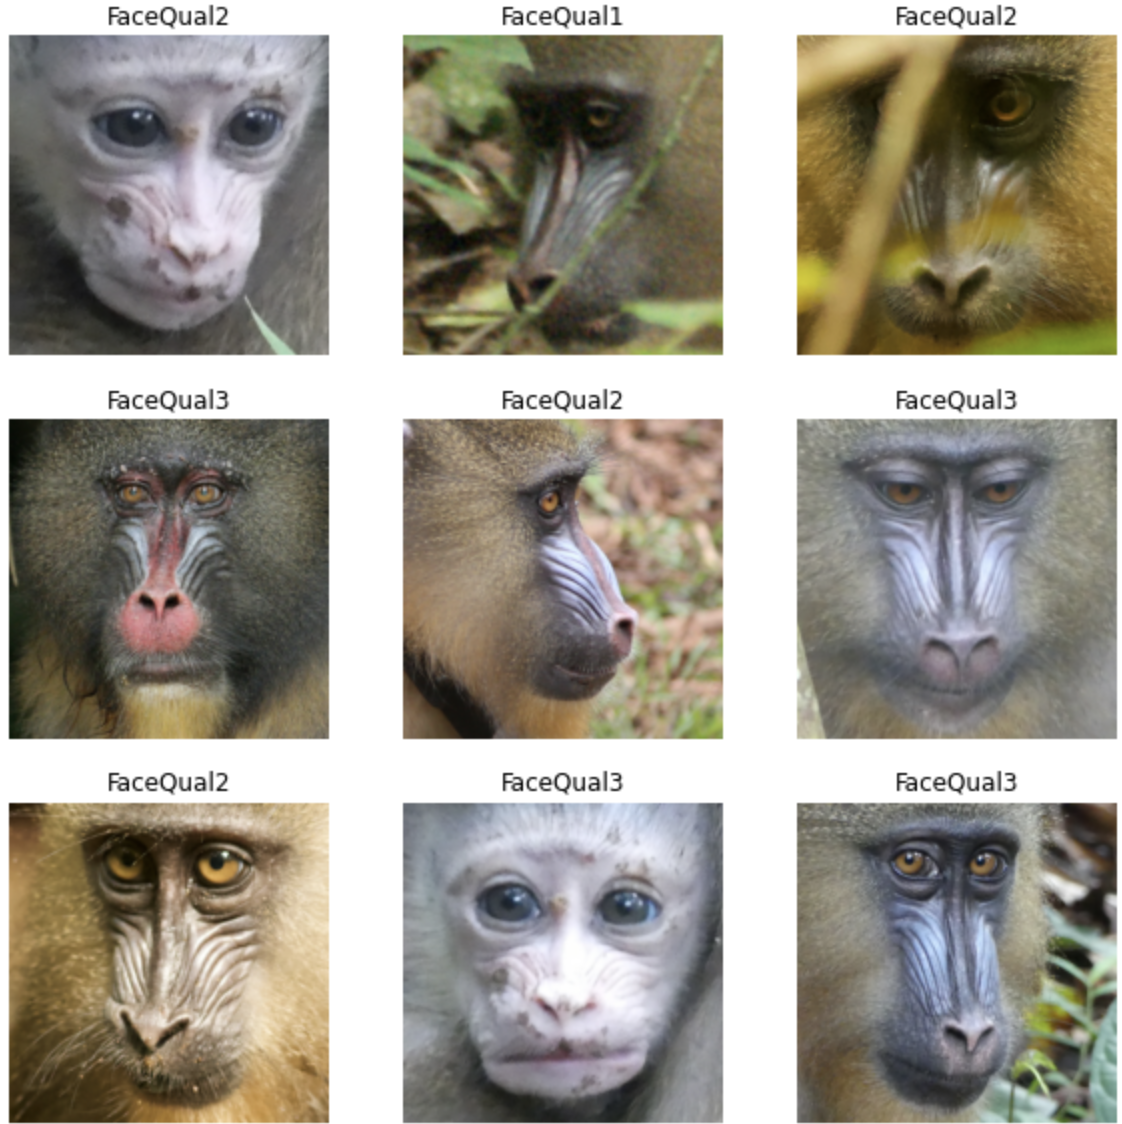
\includegraphics[width=200]{imgs/qualité/cr1/dataset.png}
\end{center}

Les premiers résultats semblent bons à première vue : 85\% d'accuracy sur une classification simple.

\begin{center}
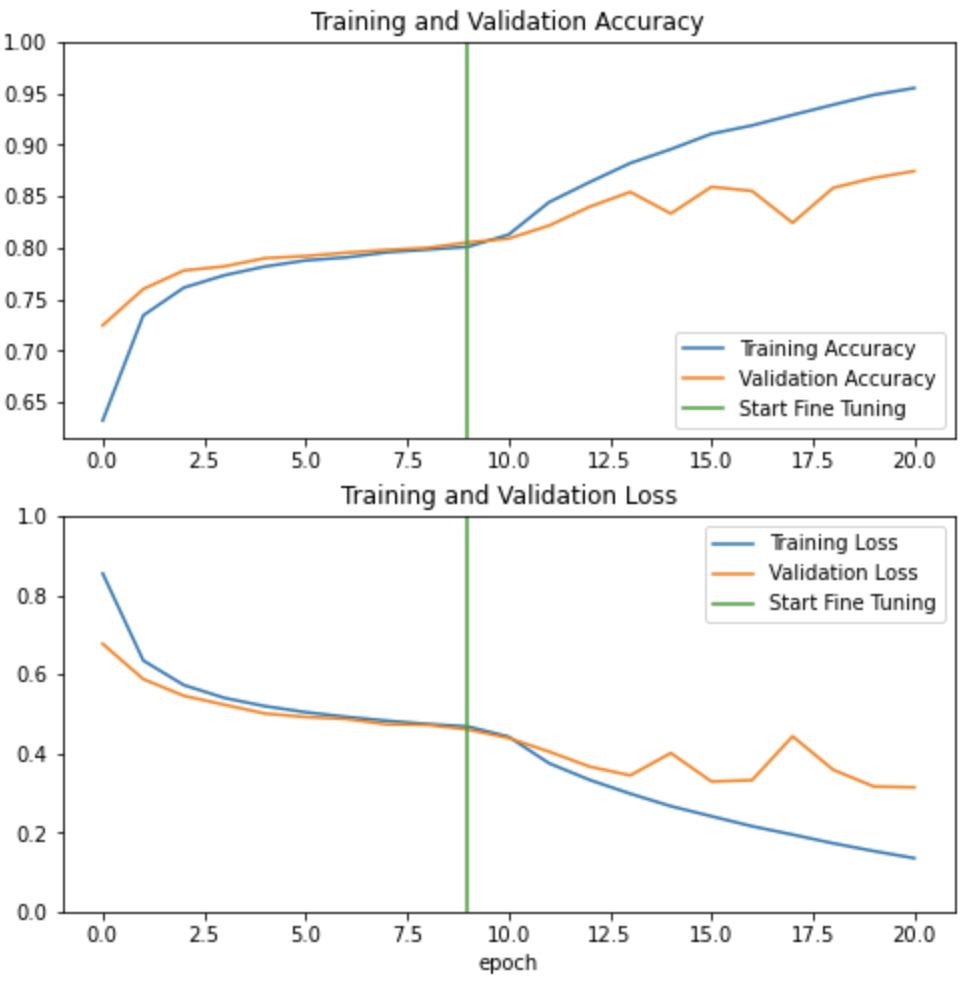
\includegraphics[width=200]{imgs/qualité/cr1/resultat1.png}
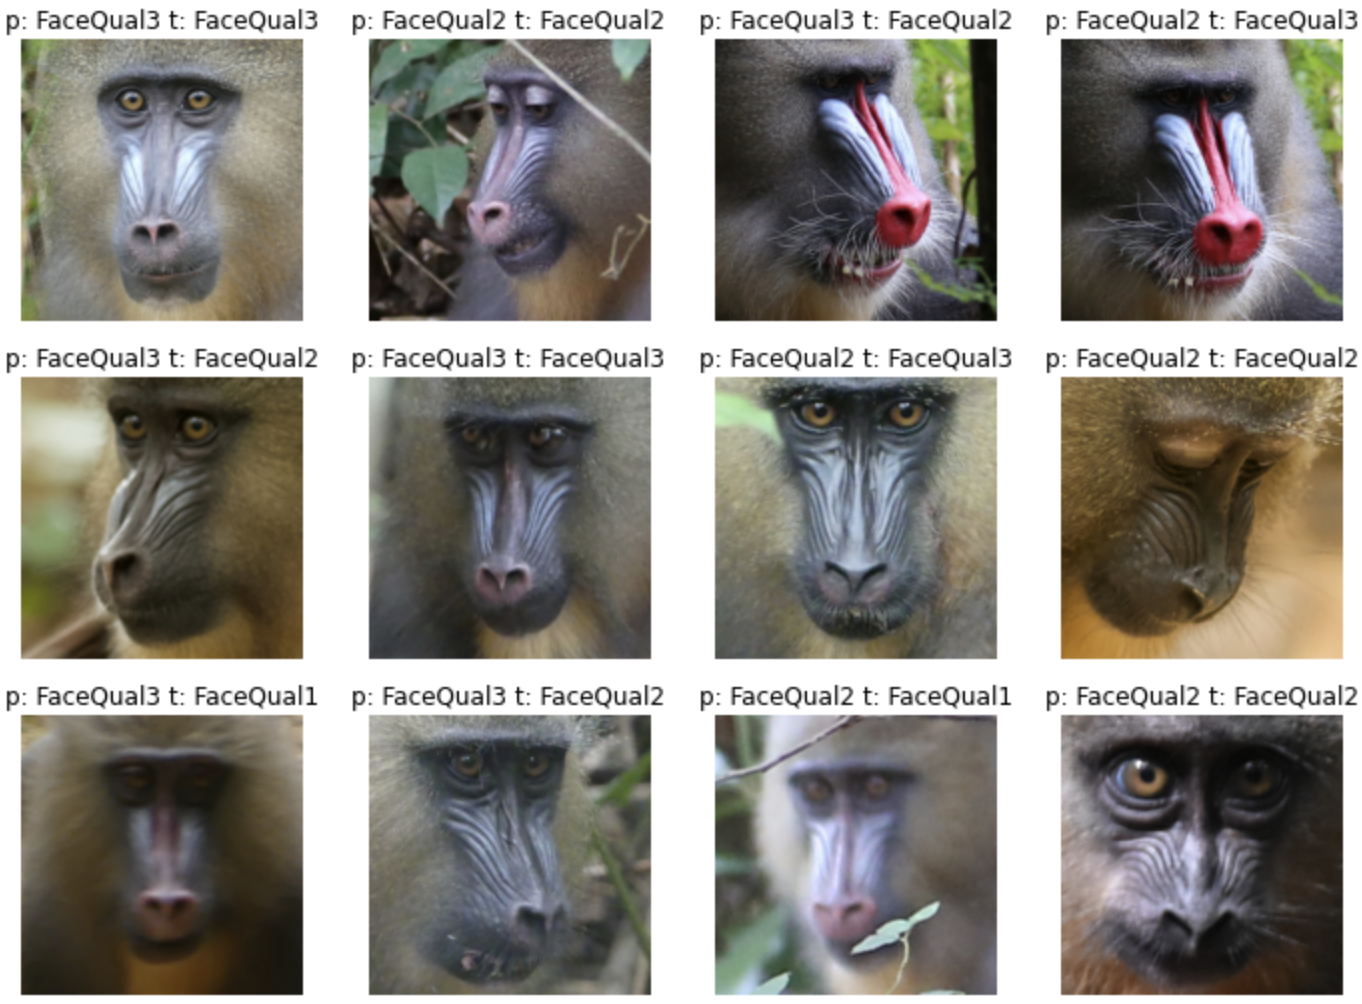
\includegraphics[width=200]{imgs/qualité/cr1/prediction1.png}
\end{center}

Mais les résultats sont trompeurs, en effet, le jeu de données est très déséquilibré, avec 10000 images de qualité FaceQual2 et 6000 de qualité FaceQual3 contre 250 et 1000 de qualité FaceQual0 et FaceQual1. Le modèle pourrait donc prédire tout le temps FaceQual2 et avoir 57\% d'accuracy par défaut.\\

Il faut donc gérer ce déséquilibre, et deux approches nous paraissent intéressantes :\\
\begin{itemize}
    \item dégrader des images de bonne qualité (downscale puis upscale et léger floutage) pour génerer des photos de mauvaises qualité (une mauvaise photo souvent a un manque de détails et/ou est flou).
    \item pondérer les classes de jeu de données pendant l'entrainement (accorder plus d'importance donc là où on aurait moins d'échantillons).
\end{itemize}

Voici un exemple de ce que pourrait être une dégradation d'images par rapport aux premières images :

\begin{center}
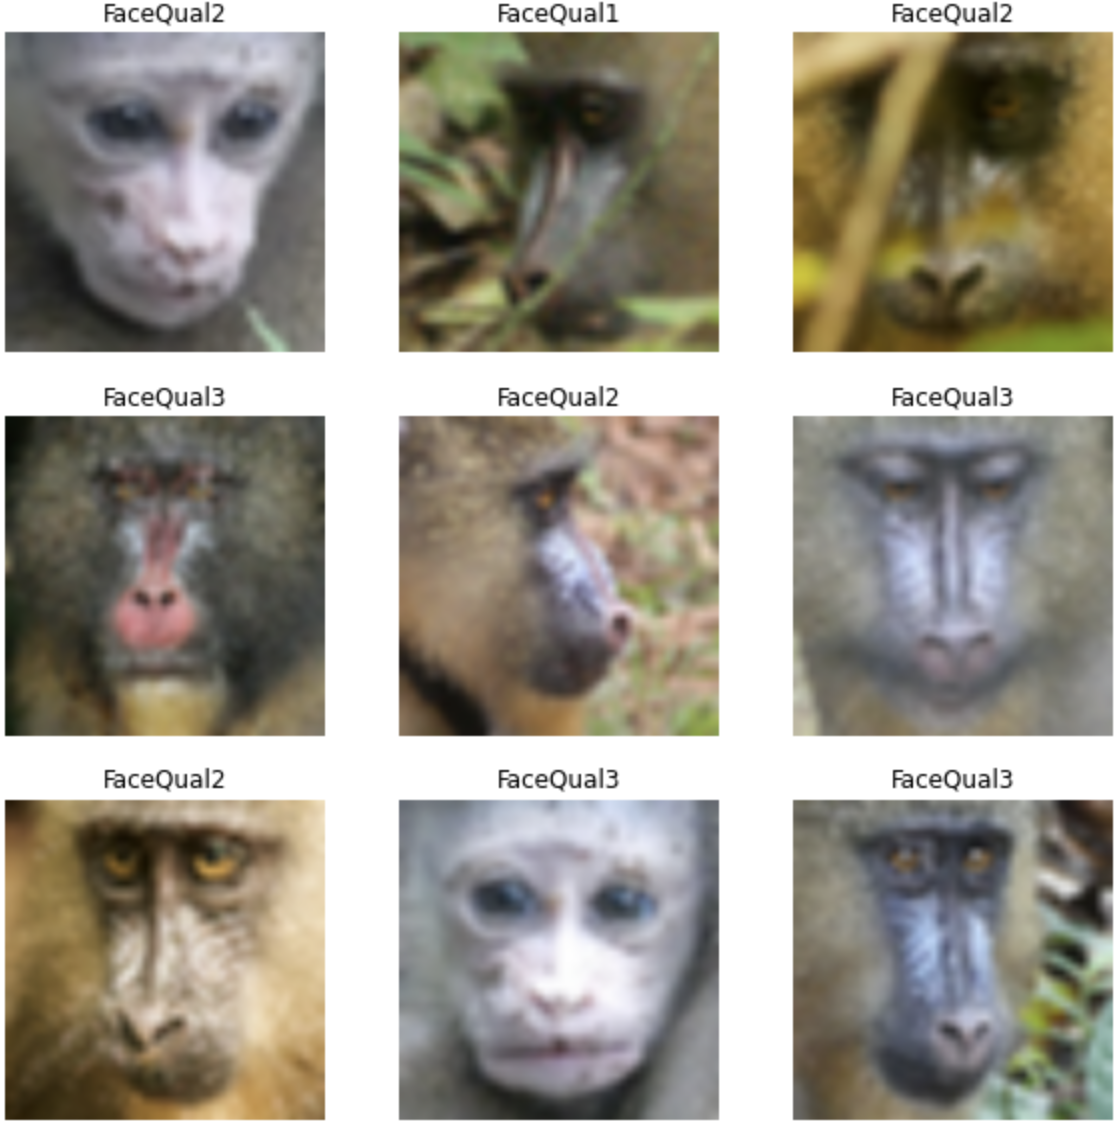
\includegraphics[width=200]{imgs/qualité/cr1/augmentation1.png}
\end{center}

Évidemment on peut faire varier le niveau de floutage et de dégradation de détails. On pourrait également imaginer appliquer un fort taux de compression JPEG ou augmenter le bruit artificiellement pour obtenir des images de basse qualité réalistes (tout cela étant des facteurs de basse qualité).\\

Il serait utile de visualiser le problème d'équilibrage par une matrice de confusion et peut être un graphe ROC. Ensuite, il faudra donc essayer d'obtenir un modèle qui fonctionne sans "tricher", avec les méthodes citées plus hauts.

\end{document}
